\documentclass{IEEEtran}

\usepackage[utf8]{inputenc}
\usepackage{graphicx}
\usepackage{amsmath}
\usepackage{siunitx}
\usepackage{listings}
\usepackage[citestyle=ieee,sorting=none,bibencoding=utf8,backend=biber]{biblatex}
\usepackage{caption}
\usepackage{subcaption}

\usepackage{algorithm}
\usepackage[noend]{algpseudocode}

\graphicspath{{images/}}
\bibliography{bibliography}
\makeatletter
\def\BState{\State\hskip-\ALG@thistlm}
\makeatother

\author{J.R. Powers-Luhn}
\title{Ridge Regression}
\date{October 16th, 2018}

\begin{document}
\maketitle

\begin{abstract}

A regularization method for linear regression is explored. A term is added to the cost function proportional 
to the magnitude of the coefficients. A scaling term, $\alpha$, adjusts the tradeoffs between model bias and 
variance. Two methods for optimizing the scaling term are examined. This method is used to generate models 
for predicting body fat percentage. The selected model is accurate to a root mean squared error of \num{4.34}.

\end{abstract}

\section{Introduction}

Least squares regression makes the assumption that its predictors are linearly independent of each other. 
If the variables are not linearly independent, then the matrix of model inputs is singular and cannot be 
inverted. In the real world, the presence of random noise precludes any two inputs being perfectly correlated, 
but this also means that small changes in the input measurements (i.e. a slightly different noise value from 
the same distribution) can have large, unpredictable effects on the coefficients from the regression model. 
Since many coefficients fit the data to within the noise present in the system, it is difficult to choose the 
correct coefficients.

One method to address this is to apply a regularization term to the cost function. By applying prior knowledge 
of the system (in this case, the fact that inputs and outputs should vary smoothly and continuously) it is 
possible to select from the ``many coefficients'' above. 

The regularization term applied in this case is the $\ell_2$ norm of the coefficients of the model. When this 
term is appropriately scaled it allows a tradeoff between the variance and bias of the model. Due to similarities 
between this method and quadratic response functions this method is known as ridge regression. \cite{hoerl1970ridge}.

\section{Methodology}

The naive solution to the linear regression problem $$\mathbf{X} \vec{b} = \vec{y}$$ is to invert $\mathrm{X}$ 
and left-multiply: $$\vec{b} = \mathbf{X}^{-1} \vec{y},$$ but this depends on how invertible X is. This is 
expressed in the condition number of X (equation \ref{eq:condition_number}, where the $\lambda$ values are the 
largest and smallest eigenvalues of $\mathbf{X}$). Large condition numbers (in excess of 100) imply that the 
matrix is nearly non-invertible and the solution will vary significantly based on the small variations caused 
by noise.

\begin{equation}
	Cond(\mathbf{X}) = \frac{\lambda_{max}}{\lambda_{min}}
	\label{eq:condition_number}
\end{equation}

By assuming that the solution to the linear regression problem should be insensitive to noise, it 
follows that the coefficients $\vec{b}$ should be small. The cost function is 
thus modified to that shown in equation \ref{eq:ridge_cost}.

\begin{equation}
	|| \vec{y} - \mathbf{X} \vec{b} ||_2 + \alpha^2 || \vec{b} ||_2
	\label{eq:ridge_cost}
\end{equation}

The derivative of this cost function is taken in order to find the value of $\vec{b}$ that minimizes 
it, leading to (after multiplying the original equation by the transpose of $\mathbf{X}$ to get a 
square matrix) equation \ref{eq:ridge_solution}.

\begin{equation}
	\vec{b} = (\mathbf{X}^T \mathbf{X} + \alpha^2 \mathbf{I})^{-1} \mathbf{X}^T \vec{y}
	\label{eq:ridge_solution}
\end{equation}

This creates an inherent tradeoff between variance and bias. If $\alpha$ is too small, the model will 
have a high variance and be subject to noise in the data. If $\alpha$ is too large, the model will have 
a high bias--it will be very stable, but will not fit the data well. Several methods exist for selecting 
$\alpha$; two are described below.

In order to examine this method, a simulated dataset was generated consisting of one hundred measurements 
each of two perfectly correlated input ``measurements'', $x_1$ and $x_2$. $x_1$ and $x_2$ differed in scale, 
but were otherwise identical. Uniformly distributed noise was added to each measurement. Output values were 
generated from the equation $y = 0.1 x_1 + 0.9 x_2$ with additional uniform noise added.

The data were first split into training, test, and validation sets. Each variable (corresponding to a 
column in the input matrix) is scaled to be mean centered with unit variance. The output variables are 
also scaled in the same way. Since the regularization term penalizes large coefficients, scaling the 
variables removes the dependence on the units and puts all the coefficients on the same playing field.

\subsection{Leave One Out Cross Validation}
One method of determining the best value for $\alpha$ is to apply equation \ref{eq:ridge_solution} to 
all samples in the training set except one, which is used to determine the error. This is repeated with a 
different sample used to determine the error and the first sample returned to the training set. This process
is repeated until every sample has been used to determine error once and used to solve for $\vec{b}$ $n-1$ 
times, where $n$ is the number of samples in the training set. The error values from each calculation are 
averaged to produce a single value. This is repeated for each candidate value for $\alpha$. The value of
$\alpha$ which results in the smallest average error is selected as the best.

Applying this method yielded an $\alpha$ value of \num{0.24}, corresponding to a test RMSE of \num{0.30}.

\subsection{L-curve} \label{ss:L-curve}
An optimal value for $\alpha$ can also be determined graphically. Ridge regression is a tradeoff 
between a desire for small coefficients and small error. By plotting these terms against each other 
for a variety of $\alpha$ values it is possible to measure which $\alpha$ minimizes both of these. 

To show this, ridge regression models were again generated for a variety of candidate $\alpha$. The norm of 
the coefficients (figure \ref{fig:norm_b_vs_alpha}) and the root mean squared error (\ref{fig:rmse_vs_alpha}) 
for each model was calculated using the training set. 

\begin{centering}
\begin{figure}
\centering
\begin{center}
	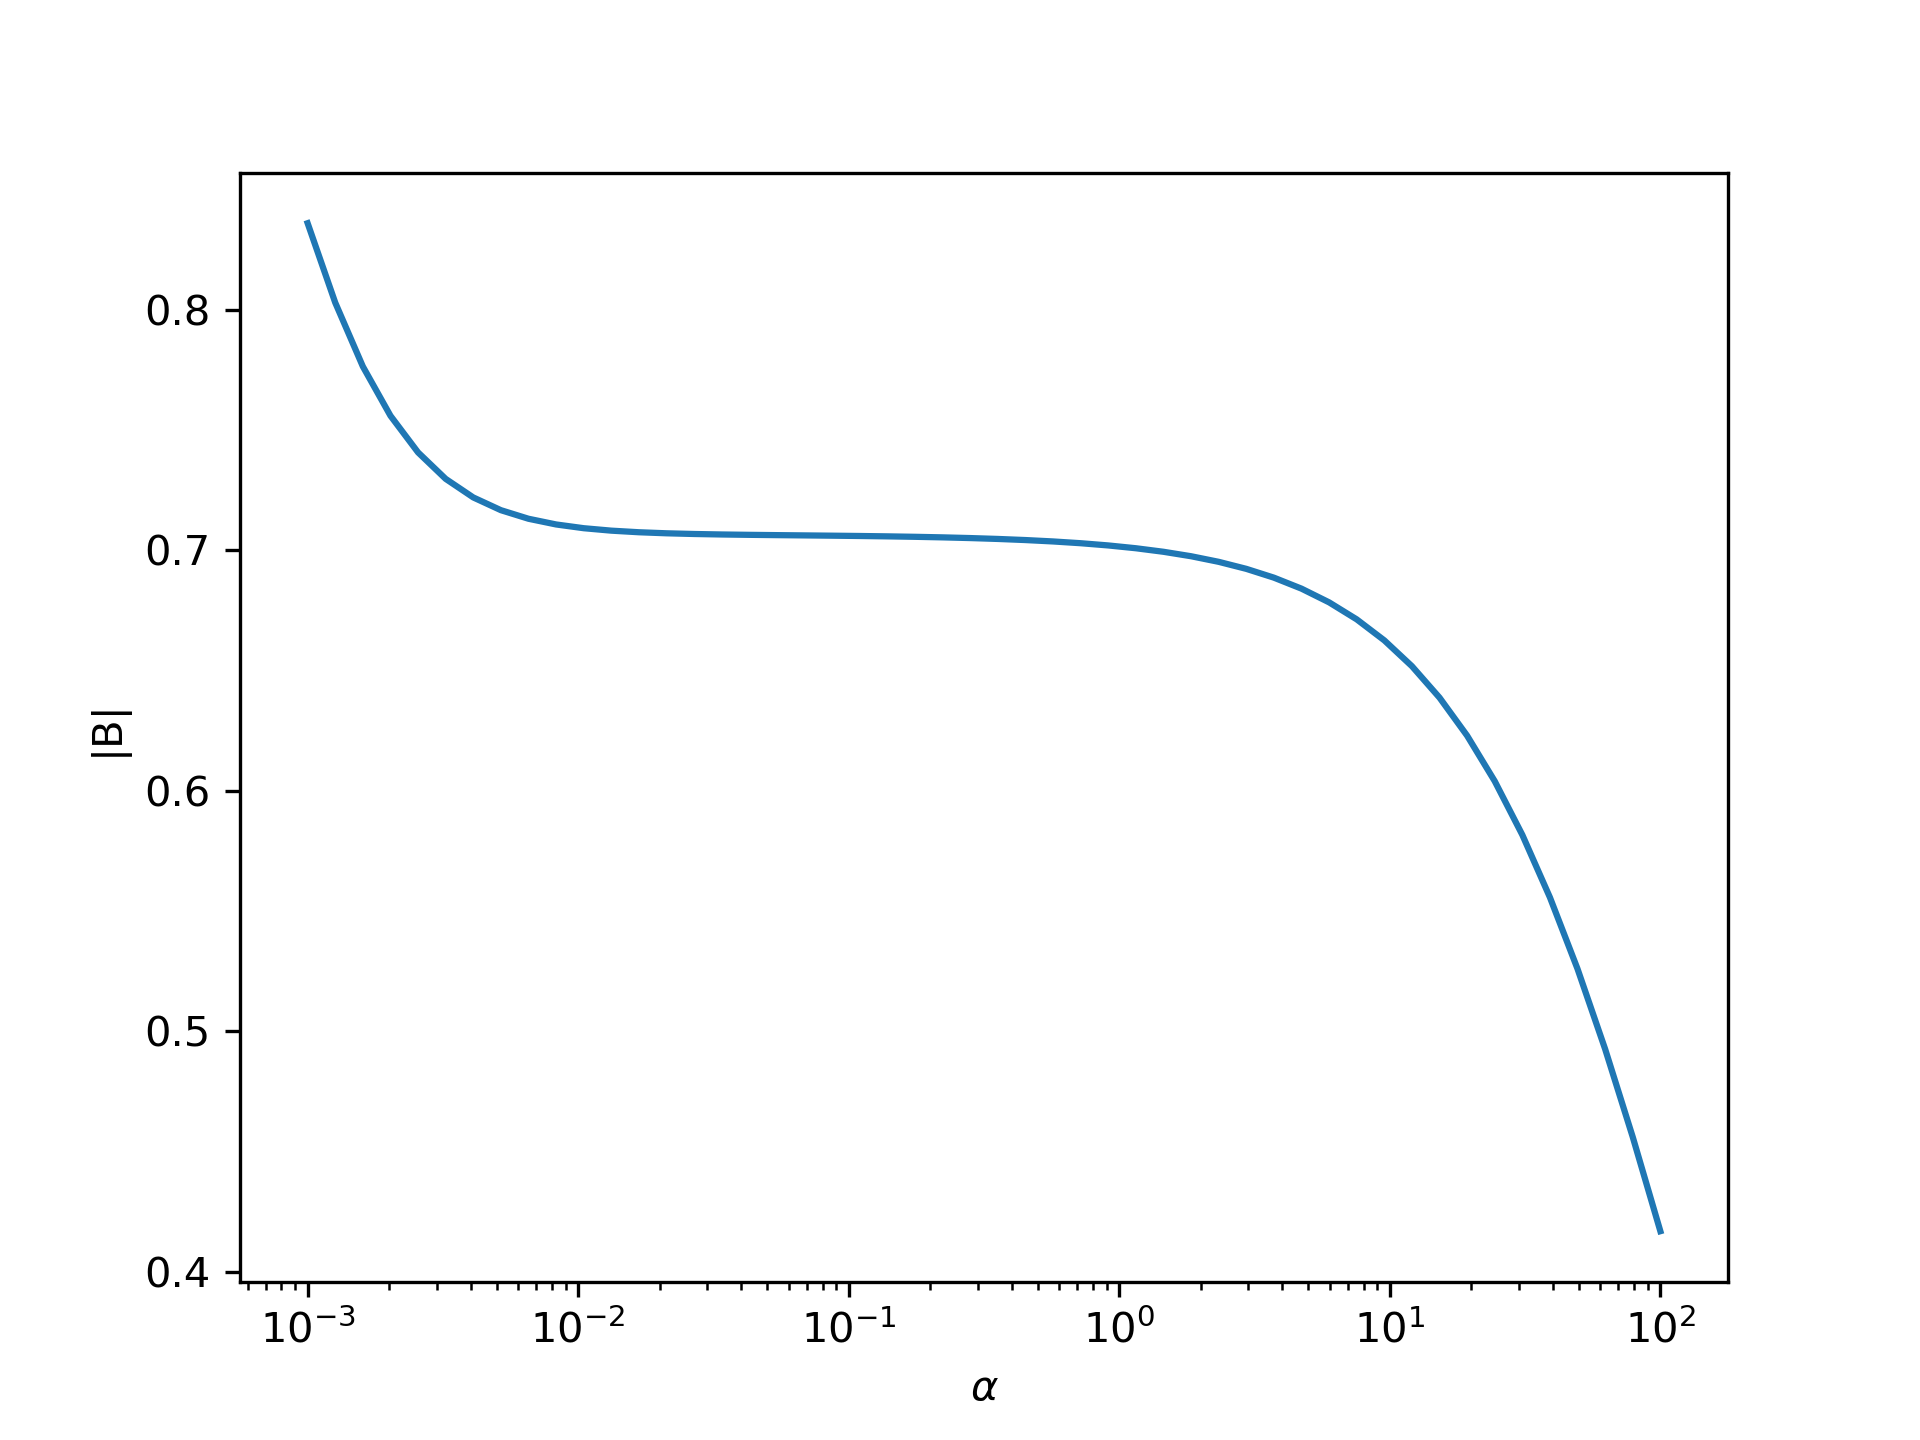
\includegraphics[width=0.48\textwidth]{norm_b_vs_alpha}
	\caption{Small values of $\alpha<<\lambda_{min}$ allow large coefficients; 
			 $\alpha ~ \lambda_{min}$ introduces a trade-off region with relatively stable models; 
			 values of $\alpha >> \lambda_{min}$ cause vanishingly small coefficients (and high bias).
			 \label{fig:norm_b_vs_alpha}}
\end{center}
\end{figure}
\end{centering}

\begin{centering}
\begin{figure}
\centering
\begin{center}
	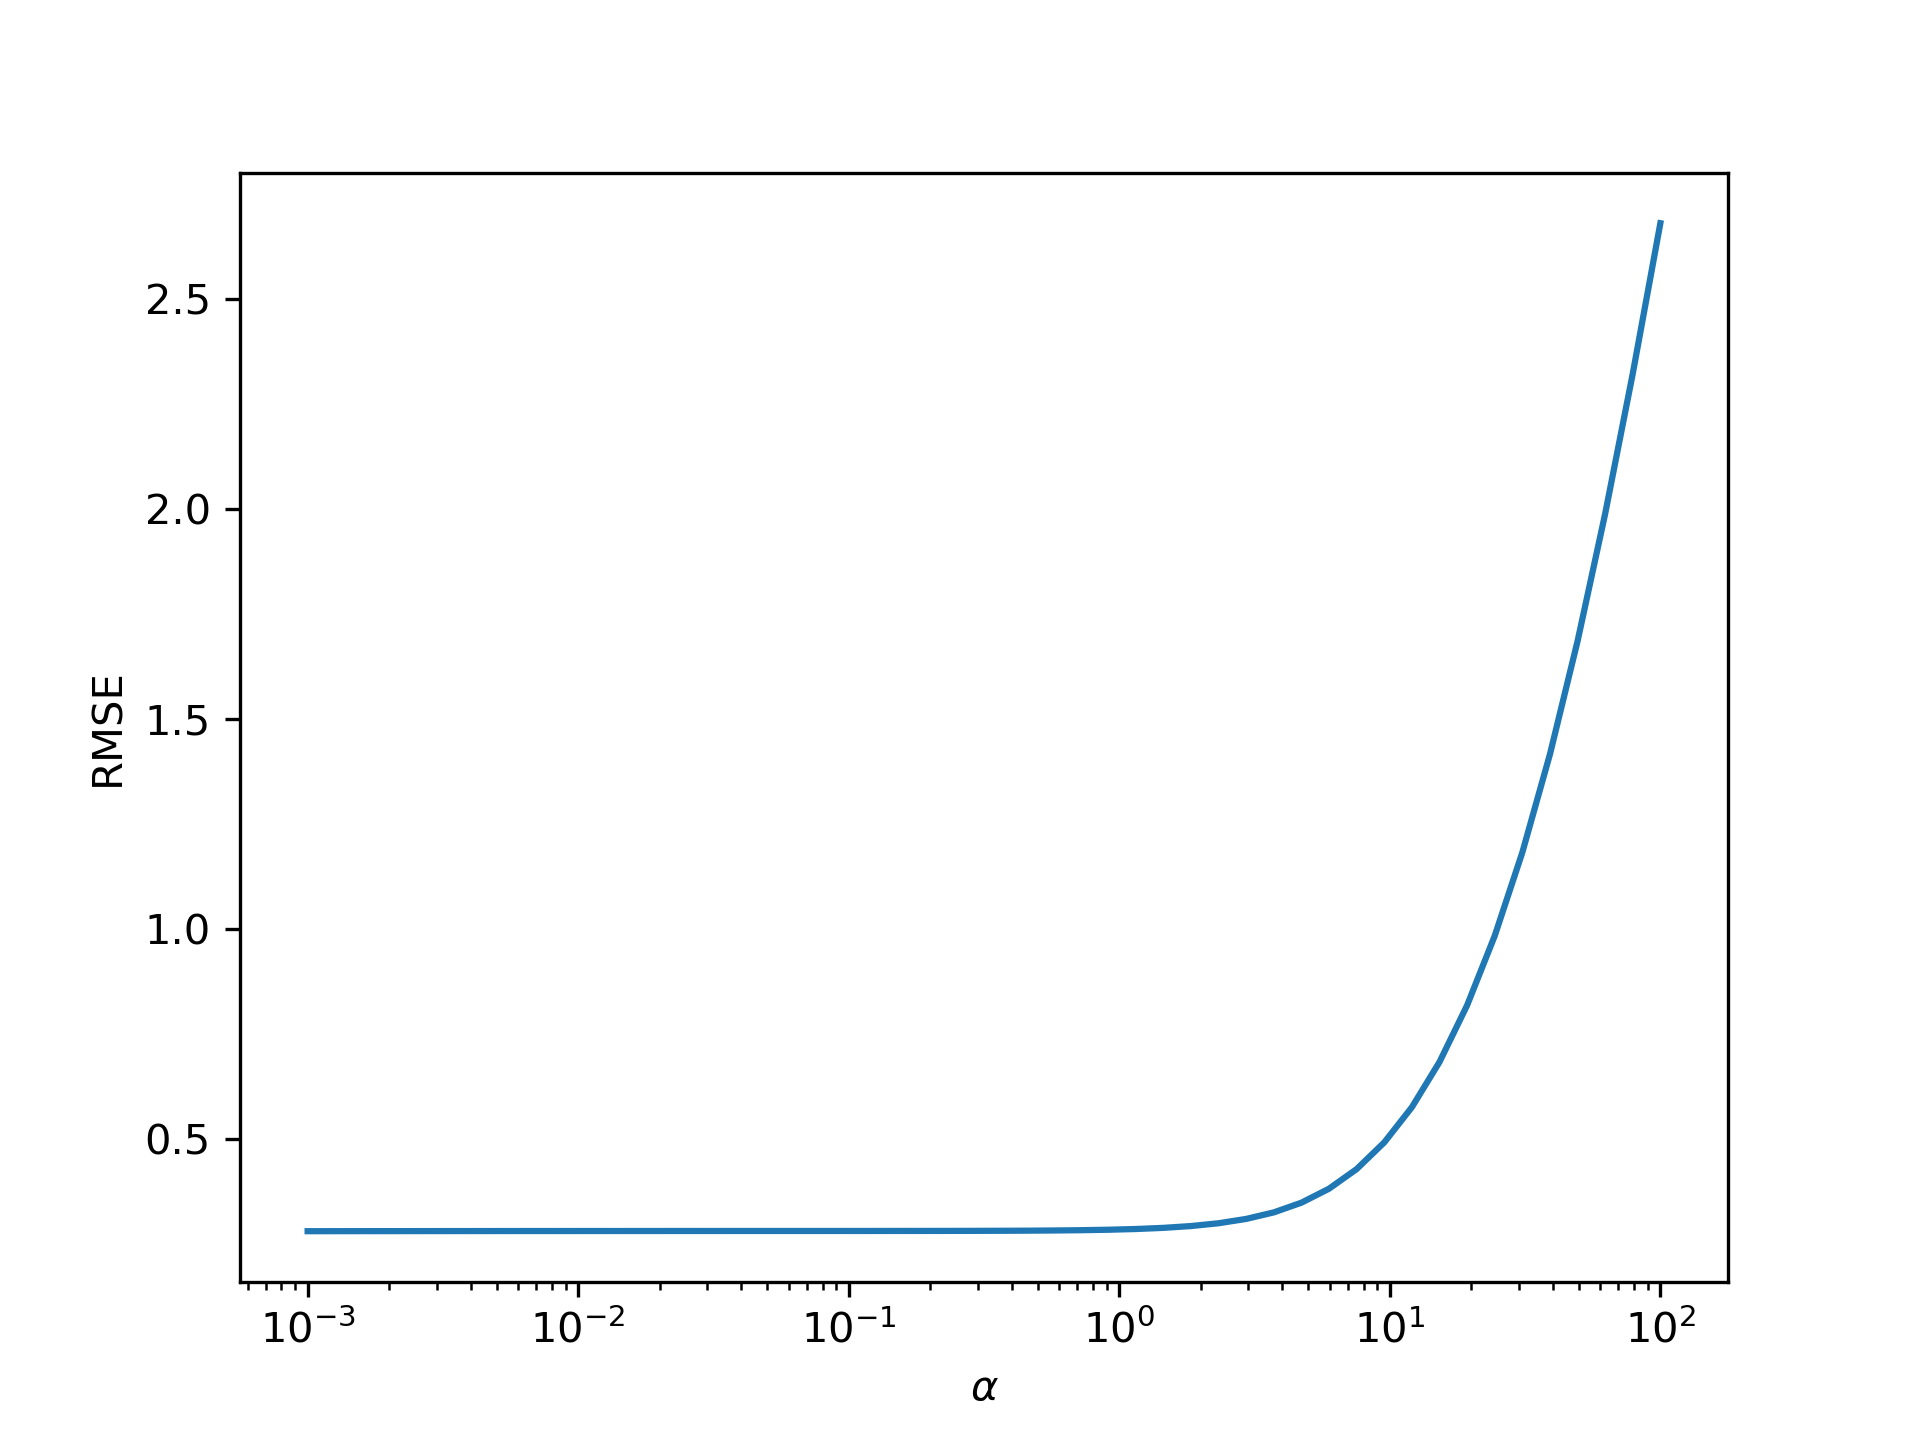
\includegraphics[width=0.48\textwidth]{rmse_vs_alpha}
	\caption{$\alpha$ has little impact on RMSE until it nears the smallest eigenvalue of $\mathbf{X}^T 
	         \mathbf{X}$. When it exceeds this eigenvalue, the model becomes more biased and RMSE increases.
	         \label{fig:rmse_vs_alpha}}
\end{center}
\end{figure}
\end{centering}

When the norm of the model coefficients and RMSE are plotted against each other (see figure 
\ref{fig:norm_b_vs_rmse}) the point of closest approach to the origin can be measured. The $\alpha$ value 
corresponding to this point is selected for the best model. 

\begin{figure}
     \centering
     \begin{subfigure}[t]{0.24\textwidth}
         \centering
         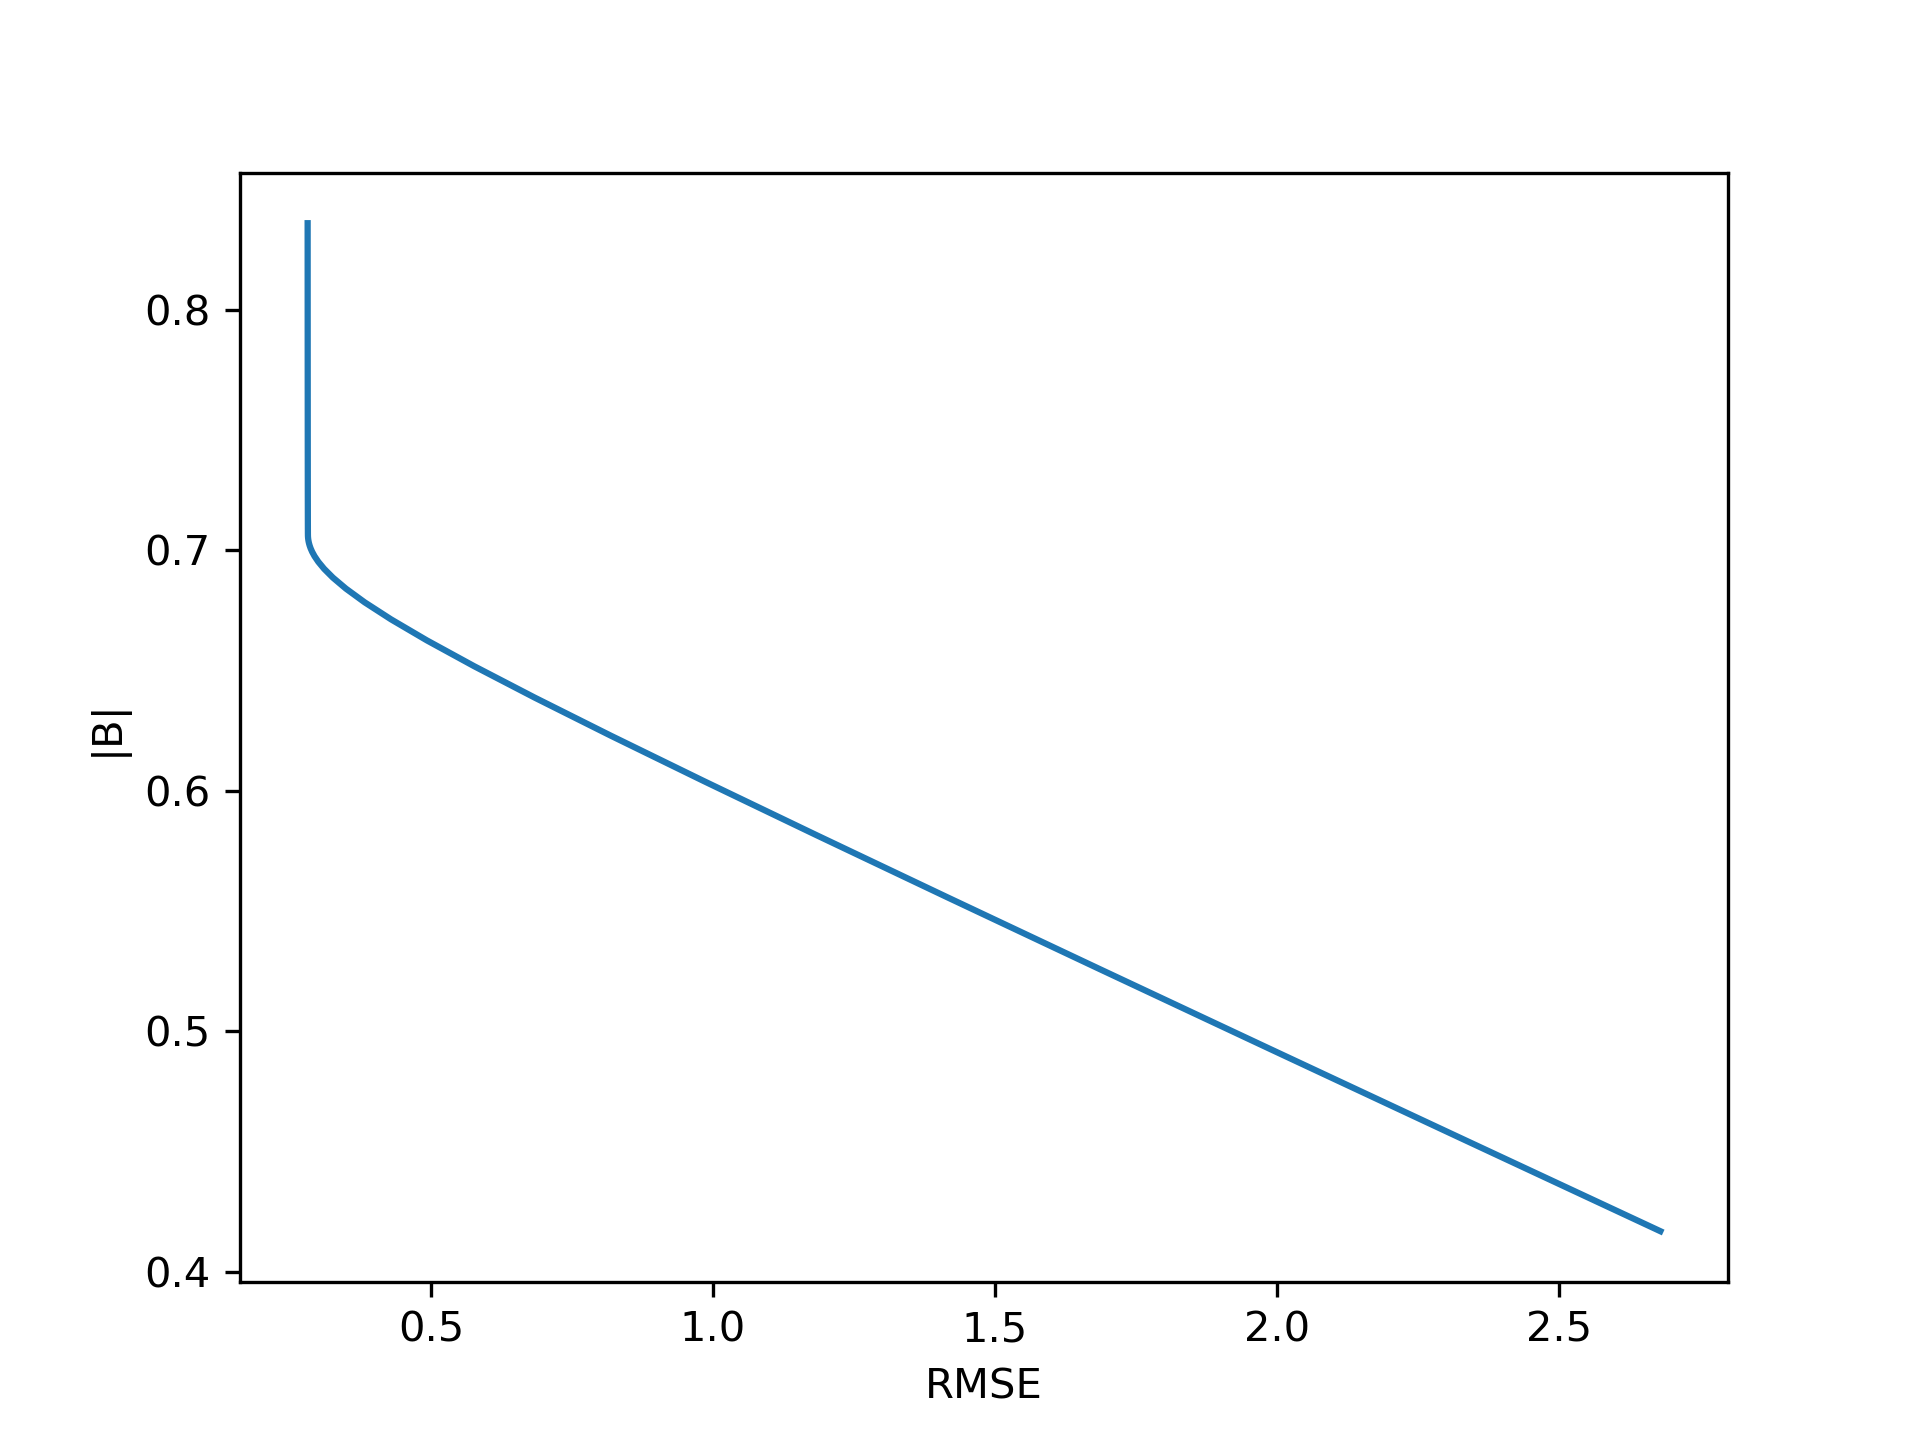
\includegraphics[width=\textwidth]{norm_b_vs_rmse}
         \caption{$L_2$ norm of coefficients vs RMSE}
         \label{fig:y equals x}
     \end{subfigure}
     \hfill
     \begin{subfigure}[t]{0.24\textwidth}
         \centering
         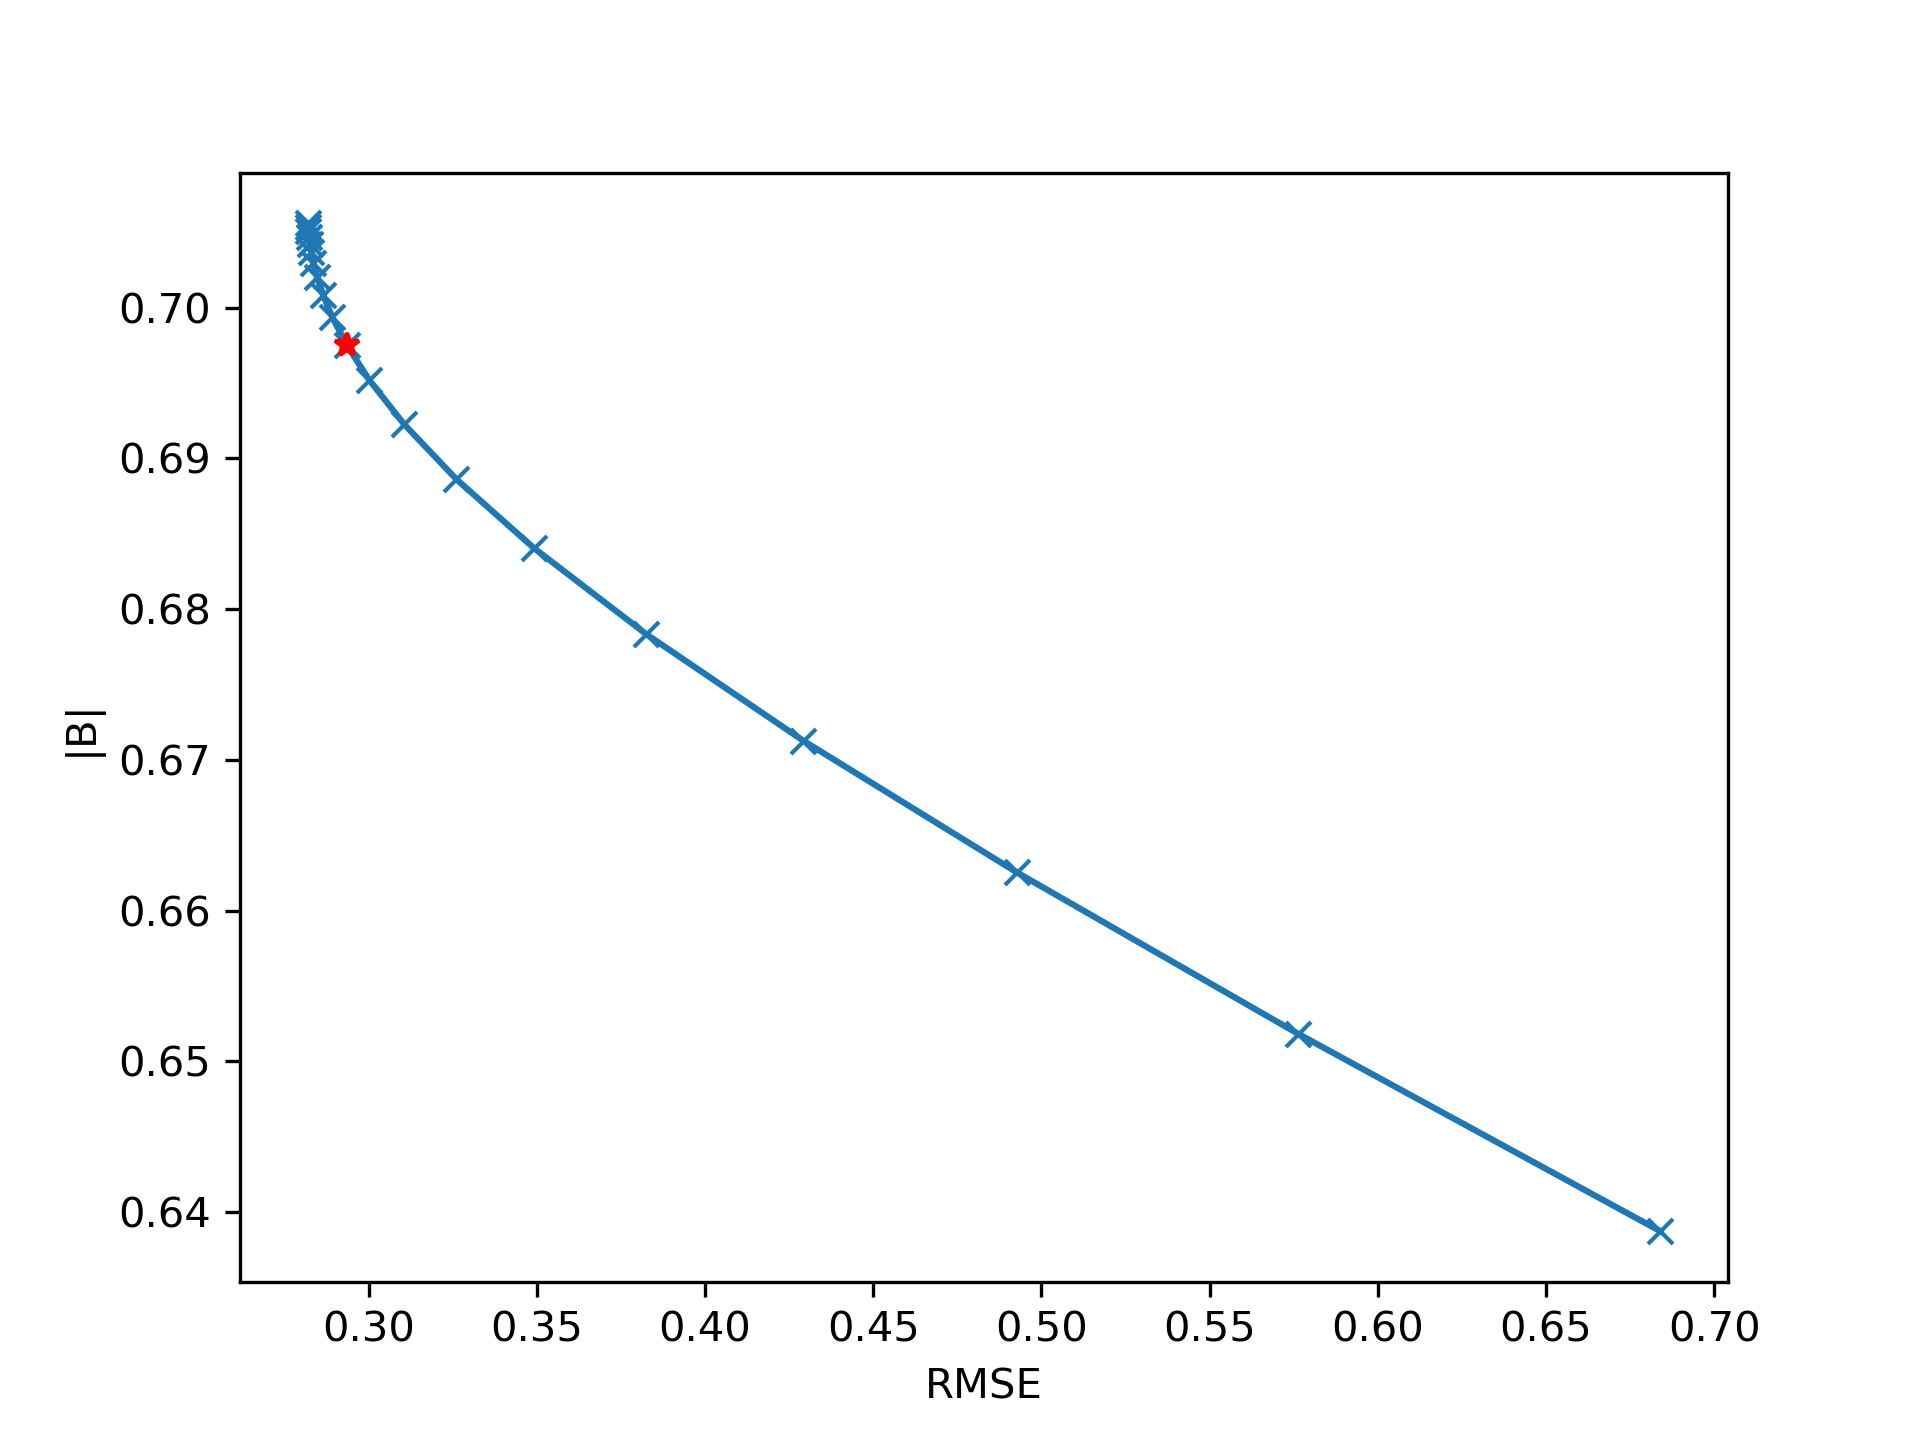
\includegraphics[width=\textwidth]{norm_b_vs_rmse_zoomed}
         \caption{Close zoom on elbow region}
         \label{fig:three sin x}
     \end{subfigure}
     \hfill
     \caption{The point on the plot of $||\vec{b}||$ vs RMSE closest to the origin is the best compromise between
     		  model bias and variance.}
     \label{fig:norm_b_vs_rmse}
\end{figure}

Using this approach, an $\alpha$ value of \num{1.84} was selected. This model had a test error of \num{0.31}.

\subsection{Condition Number}
Because these data were highly linearly dependent, the condition number was high, with a value of 
\num{2.1e6}. Standardizing the data reduced this somewhat (to \num{2.6e5}), but still high. By adding the 
$\alpha^2$ term, the condition number becomes $$ Cond(\mathbf{X} ) = \frac{\lambda_{max} + \alpha}
{\lambda_{min} + \alpha}. $$ This disproportionately affects the denominator, pushing the condition number 
down. This also sets the scale of the $\alpha$ value--if $\alpha << \lambda_{min}$, ridge regression acts 
essentially like least squares regression. If $\alpha >> \lambda_{min}$, the model will have a high bias 
and will not fit the data well. $\alpha$ should be on a similar scale to the smallest eigenvalue of 
$\mathbf{X}^T \mathbf{X}$. With the $\alpha$ selected in section \ref{ss:L-curve}, this results in a 
condition number of \num{79}, below the rule-of-thumb value of \num{100}.

\subsection{Body Composition}
A dataset of body measurements (body fat percentage, age, weight, height, adiposity index, and ten 
circumference measurements) was obtained \cite{Penrose1985}. Ridge regression was used to generate models to 
predict body fat percentage from the other predictor variables using the two methods described above to select 
the hyperparameter $\alpha$.

\section{Results}

\subsection{Leave One Out (LOO) Cross Validation}
The value of $\alpha$ that minimized the mean RMSE from the cross-validated segments was determined to be 
\num{0.10}. This corresponded to an RMSE of \num{3.83} on the test set.

\subsection{L-curve} \label{ss:Results L-Curve}
The value of $\alpha$ that minimized the $\ell_2$ norm of $\vec{b}$ and RMSE was determined to be \num{2.81}. 
This gave a test set error of \num{3.86}.

%\begin{centering}
%\begin{figure}
%\centering
%\begin{center}
%	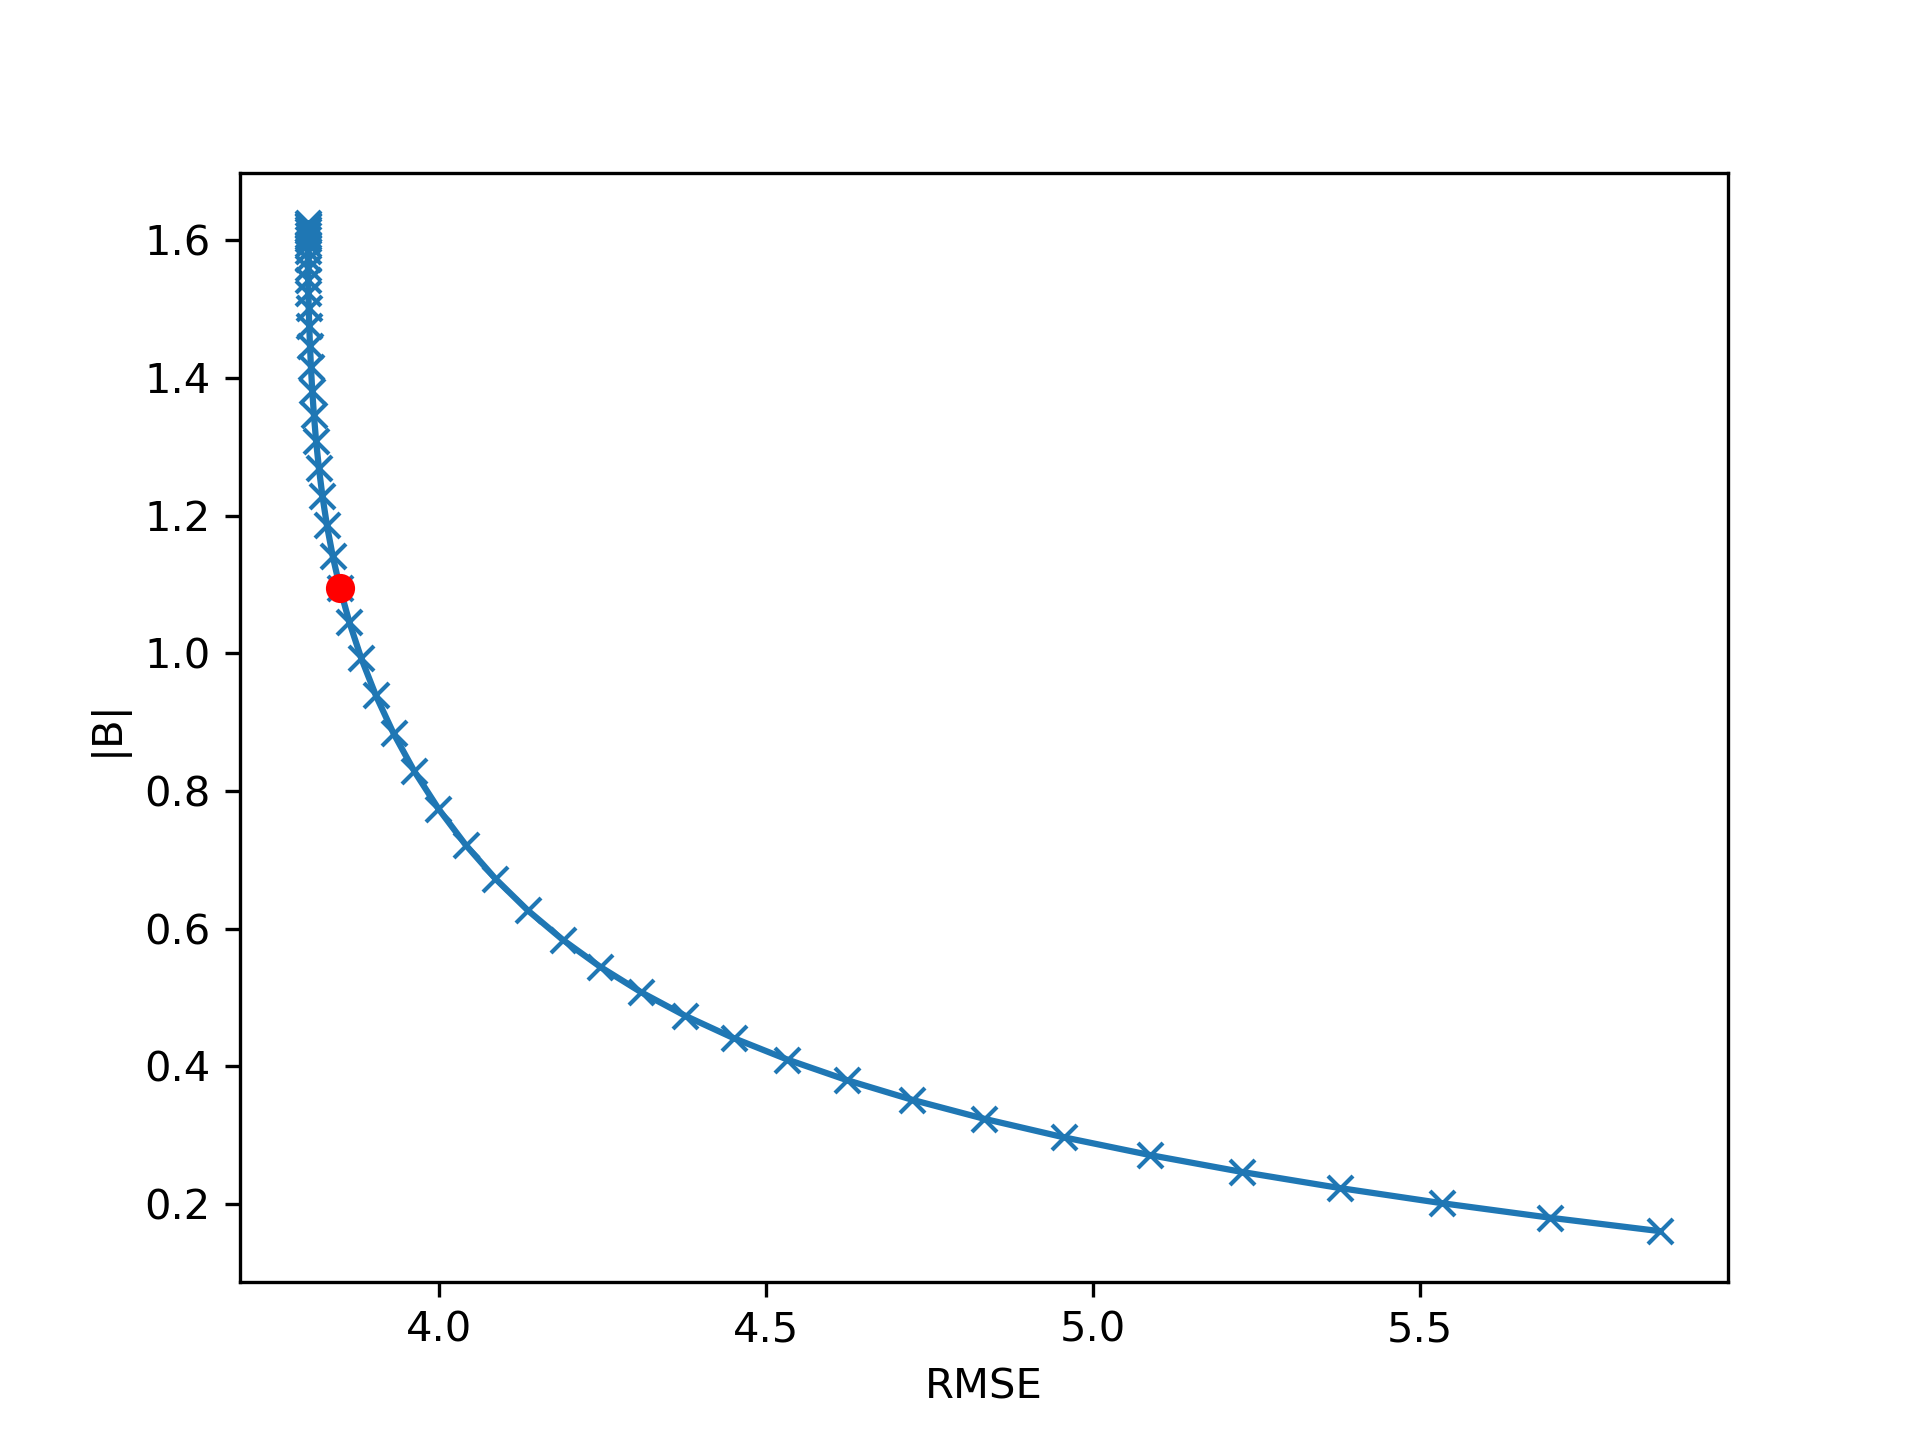
\includegraphics[width=0.48\textwidth]{bw_norm_b_vs_rmse_with_best_alpha}
%	\caption{L-curve optimization of $\alpha$
%	         \label{fig:bw_norm_b_vs_rmse_with_best_alpha}}
%\end{center}
%\end{figure}
%\end{centering}

\subsection{Model Stability}
Initially the matrix $\mathbf{X}^T \mathbf{X}$ had a condition number of \num{3.7e5}. Standardizing the training 
data reduced this to \num{2056}--a significant effect, likely because of the very different units and scales of 
the predictors. Applying the $\alpha$ value determined in section \ref{ss:Results L-Curve} reduced this an 
additional order of magnitude to \num{470}, still not below the threshold value of \num{100}.

\subsection{Model Selection}
The model that was selected was that produced by the L-curve method. Its performance was not significantly 
different from the model produced using the LOO method and the larger $\alpha$ value should result in greater 
stability. Both models significantly improved on the least squares model, which had an RMSE of \num{19.35}.

The selected model was evaluated on the validation set data, producing an RMSE of \num{4.34}.

\section{Conclusions}

A model was generated to predict body fat percentage from body composition predictors. The error of this model was \num{4.34}. This was comparable to the error produced by a partial least squares model (\num{4.35}) and showed improvement over principal component regression (\num{4.72}) and a best-guess linear regression (\num{4.79}). Further, the linear model required the calculation of inverse terms while the ridge regression was both straightforward to calculate (unlike PLS, no iterative algorithms were necessary) and did not require non-linear terms. Two methods of selecting the hyperparameter $\alpha$ were examined. Leave one out cross validation was easy to understand but computationally expensive and might be prohibitive for large datasets. Variations on this method (e.g. ``Leave K out'') are worth exploring if they lead to stable results. The L-curve method of determining $\alpha$ clearly demonstrates the bias/variance trade, making it attractive if potentially subjective. 

\printbibliography

\onecolumn
\section{Appendix}
Python code used to perform calculations and generate graphics.
\lstset{frame=single}
\lstinputlisting[language=Python]{hw06_sim.py}

\end{document}